\textbf{Photoluminescence} is the emission of light by the excited molecules and/or 
molecule clusters. Here we are intended to observe photon emission from the defects 
within crystalline structures such as diamond and cubic boron nitride. Given that these
materials known to be opaque in visible light range, we are building a \textbf{reflecting 
light microscope}[refhere]. Although wide-field excitation (similar to epifluorescence 
[refhere]) based emission measurements from an ensemble of defects have their own 
importance in characterization, we pursue investigating properties of individual defects/
emitters. This requires our reflecting light microscope to be a \textbf{confocal system}.  

\subsection{Reflecting Light Microscopes Overview}
On typical an upright or inverted microscope, illumination light comes from a direction 
relative to sample surface, while the collection or imaging is done in the opposite direction. 
Therefore in terms of optical components, illumination and imaging sides differ in those
systems. For example in illumination side a special lens called \textbf{Condenser} focuses
the light on to the sample while in the imaging side another special lens called \textbf{
Objective} lens collects the light coming from the sample. These special lenses and the
typical upright and inverted microscope configurations are shown in Figure\ref{fig:CondenserAndObjective}.

\begin{figure}[H]
	\centering
	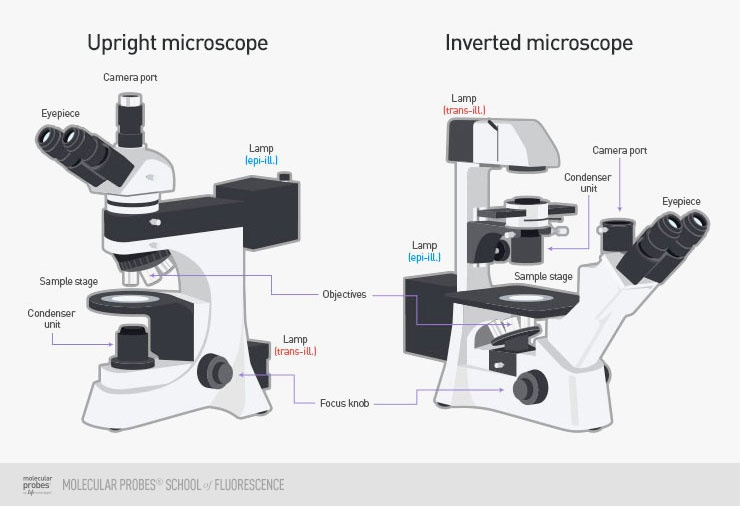
\includegraphics[angle=0,origin=c,width = 1.0\linewidth]{Section_Microscope/Figures/CondenserAndObjective.jpg}
	\caption{A typical upright (\textbf{left}) and an inverted (\textbf{right}) microscope 
		structures indicating the positions of special lenses (\textbf{Condenser and objective}).}
	\label{fig:CondenserAndObjective}
\end{figure}

On the other hand, in a reflecting microscope illumination and imaging are done through the
same optical path or by same optics. As it is shown in Figure\ref{fig:ReflectingMicroscope},
shared optical path allows one (1) additional port for imaging and/or illuminating the sample
on a typical reflecting microscope. This port is very frequently assigned to white-light
(\textbf{bright-field}) imaging through a camera, so it is called the camera port. As a result
any additional illumination and/or imaging on top of the default system, require a custom
design optical system with the ability to finely couple with the existing microscope.

\begin{figure}[H]
	\centering
	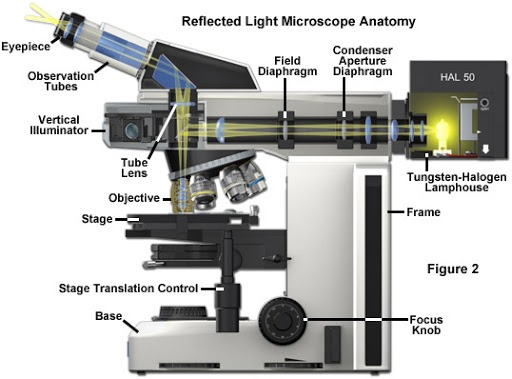
\includegraphics[angle=0,origin=c,width = 1.0\linewidth]{Section_Microscope/Figures/ReflectingMicroscope.jpeg}
	\caption{Schematics of a typical reflecting microscope with light path and internal 
		optical components.}
	\label{fig:ReflectingMicroscope}
\end{figure}

\subsection{Confocal Systems Overview}
A \textbf{confocal system} is an imaging system that utilizes a spatial filter
(or simply a pinhole) before the imaging component for strictly matching the illumination 
volume with the observation volume as it is shown in Figure\ref{fig:WidefieldVsConfocal}. Because 
of very likely chromatic aberrations \footnote{\url{https://www.microscopyu.com/tutorials/chromatic}} 
through the imaging components, usually illumination is done by a single color light source such as 
a laser. The pinhole suppresses the out-of-excitation volume light dramatically, so it increases 
the resolution of imaging system, Figure\ref{fig:WidefieldVsConfocalResolution}. 

\begin{figure}[H]
	\centering
	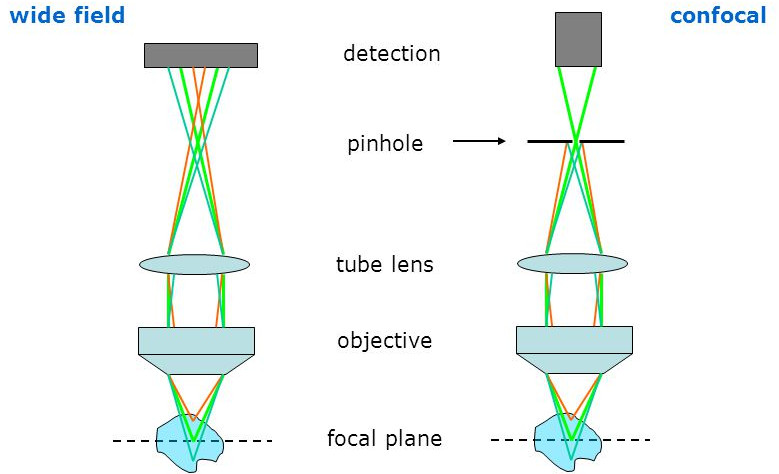
\includegraphics[angle=0,origin=c,width = 1.0\linewidth]{Section_Microscope/Figures/Confocal_microscopy_Basic_principle1.jpg}
	\caption{Simplified structure of a typical widefield (\textbf{left}) and a confocal (\textbf{right})
		imaging system  with spatial filter. ADD REF-FOOTNOTE HERE!!!}
	\label{fig:WidefieldVsConfocal}
\end{figure}

\begin{figure}[H]
	\centering
	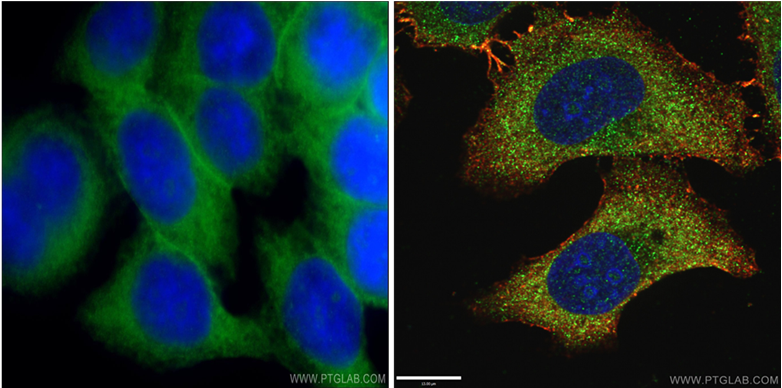
\includegraphics[angle=0,origin=c,width = 1.0\linewidth]{Section_Microscope/Figures/EpiVsConfocal1.png}
	\caption{Imaging of HeLa cells with a typical widefield (\textbf{left}) and with a confocal 
		(\textbf{right}) imaging system. ADD REF-FOOTNOTE HERE!!!}
	\label{fig:WidefieldVsConfocalResolution}
\end{figure}

Microscope manufacturers very frequently incorporate additional openings (called \textbf{microscope ports})
on sides, front and even at the bottom of microscope bodies which allows the operator to 
couple additional imaging and illumination systems into the microscope. Although this is 
a very common practice in the case of transmission microscopes (upright and inverted as well),
reflecting microscopes usually don't have these additional ports, Figure\ref{fig:ReflectingMicroscope}. 
Because of missing ports, turning a reflecting microscope is considerably harder into 
a confocal system compared to transmission microscopes. 

\subsection{Confocal Reflecting Light Microscope for PL Measurements}

Our goal is to observe emission from excited lattice-defects in solids like boron 
nitride(BN) and diamond[REF HERE!!!]. These materials are not particularly transparent
to visible light\footnote{\url{https://en.wikipedia.org/wiki/Boron_nitride}}. Moreover
defect formation (particularly in the case of BN) is induced by ion bombardment, so
neither the density nor spatial distribution of defects are known prior to a PL 
measurement. The lack of information on defect positions introduces the requirement 
of active search for defects within the sample volume, so a confocal imaging system 
with the capability of scanning. To overcome the refractive index issue and satisfying 
the confocality in imaging, we built a confocal reflecting light microscope as shown
in Figure\ref{fig:ConfocalReflectingMicroscopeFull}.

\begin{figure}[H]
	\centering
	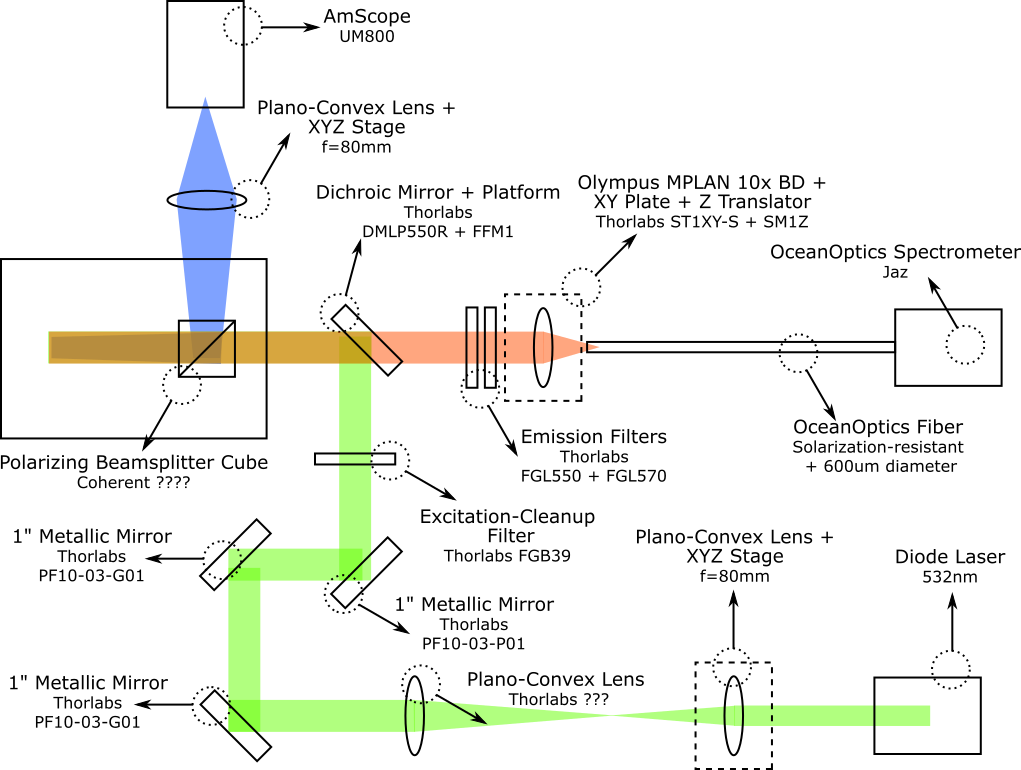
\includegraphics[angle=0,origin=c,width = 0.95\linewidth]{Section_Microscope/Figures/PL_Setup_Parts.png}
	\caption{Our homemade confocal reflecting microscope for PL measurements.}
	\label{fig:ConfocalReflectingMicroscopeFull}
\end{figure}

Although the purpose of individual parts can not be explained accurately by ignoring their 
interactions with the remaining system components, it is a common practice to divide the whole 
system into 4 essential zones for educational purposes as in Figure\ref{fig:ConfocalReflectingMicroscopeZones}. 

\begin{figure}[H]
	\centering
	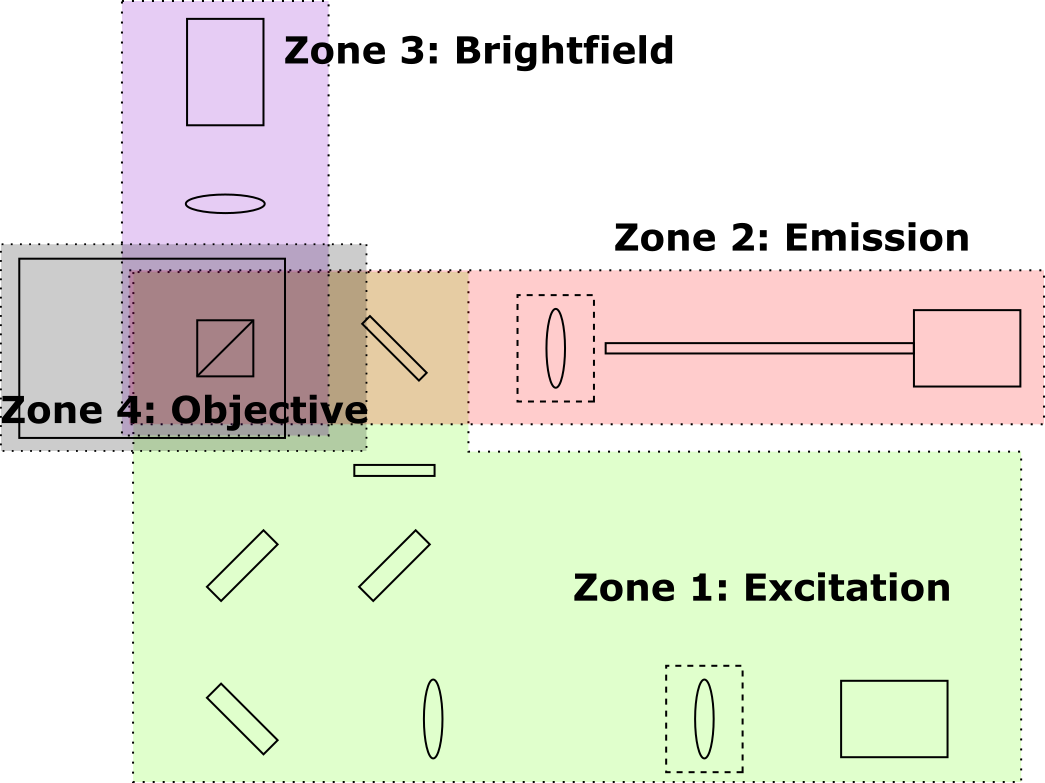
\includegraphics[angle=0,origin=c,width = 0.95\linewidth]{Section_Microscope/Figures/PL_Setup_Zones.png}
	\caption{Zones in PL microscope.}
	\label{fig:ConfocalReflectingMicroscopeZones}
\end{figure}

To briefly describe these zones;

\begin{enumerate}
	\item \textbf{Excitation, Zone 1 :} This is the zone where the excitation light is directed 
	into the microscope. The excitation source is frequently a laser, but there are systems
	which prefer broadband light sources such as UV lamps. In this zone, beam characteristics
	of excitation light (i.e. size, divergence, polarization, etc.) are adjusted to match the
	requirements imposed by other zones.

	\item \textbf{Emission, Zone 2 :} This is the zone where the emission or reflection from
	the sample is collected and analyzed by a detector. The detector can be any photon sensitive
	device (i.e. PMT, APD, CCD camera, etc.). Based on the preferred coupling mechanism in the
	sensory device, characteristics of the emission from the sample are adjusted similar to the 
	case the adjustment of excitation light.
	
	\item \textbf{Brightfield, Zone 3 :} This is the zone responsible to visual inspection of
	the sample surface and excitation/emission light profiles on the sample. Its mere purpose is
	to create an image of the sample surface and everything in near proximity on a camera and 
	allow guided tracking.
	
	\item \textbf{Objective, Zone 4 :} This is the zone where the primary imaging lens called
	objective lens resides. As a result, it is the core of the whole optical system and couples
	with all other zones. In other words, optical components in other zones are chosen/built 
	essentially for matching the objective lens to utilize the whole measurement system at its 
	maximum efficiency.
\end{enumerate}

As in any other optical system, efficiency of imaging in this system is strongly correlated with
match ratio of all these zones. Although it appears to be the Objective (Zone) 4 is the central
piece that all other zones required to be matched, there are matching requirements for among other
zones too. As a result, proper description of the microscope require deeper understanding of all
zones.

\subsubsection{Excitation, Zone 1}
In terms of the structure, this zone directly couples into Objective (Zone 4) and indirectly couples 
into Emission (Zone 2). In terms of the alignment, it directly couples into Brightfield (Zone 3).
These couplings and the required matching conditions are as following;

\paragraph{Direct coupling between Excitation and Objective}\mbox{}\\
Three essential \textbf{optical design rules} create this coupling;

\begin{enumerate}
	\item \ul{Excitation light going into the Objective has to be collimated}, so it should not be
	converging or diverging in free space for a long enough distance. On the other hand, the level of 
	collimation is very frequently not perfect, because of the real/non-ideal objective lenses.
	
	\item \ul{Propagation direction of the incoming light to the objective lens has to be 
	parallel with the surface normal of the objective lens}. A well aligned excitation beam 
	removes undesired distortions in the structure of focused light after the objective lens.
	
	\item \ul{The ratio of the diameter of excitation light and the diameter of back-aperture of the 
	objective lens (\textbf{aperture filling ratio}) has to be known and fixed to a value} 
	depending on the experimental needs (i.e. tight focus, scanning beam, etc.).
\end{enumerate}

As it is shown in the Figure\ref{fig:ConfocalReflectingMicroscopeFull}